 \documentclass{article}
\usepackage[utf8]{inputenc}

\usepackage{color}
\usepackage{url}
\usepackage[T2A]{fontenc} % enable Cyrillic fonts
\usepackage[utf8]{inputenc} % make weird characters work
\usepackage{graphicx}

\usepackage[english,serbian]{babel}

\title{Pretraživanje slika po sadržaju\\ \small{Seminarski rad u okviru kursa\\Metodologija stručnog i naučnog rada\\ Matematički fakultet}}

\author{ Božidar Mitrović, Luka Vujcić, \\ Marija Erić, Dušan Petrović }

\date{Novembar 2021}


\begin{document}

\maketitle

\abstract{
Multimedijalna analiza sadržaja se primenjuje u različitim problemima kompjuterske vizije, a digitalne slike čine veliki deo multimedijalnog sadržaja. U poslednjim godinama, kompleksnost multimedijalnih sadržaja (posebno slika) je eksponencijalno porasla. Više od milion slika dnevno dolazi do platformi poput Fejsbuka, Tvitera i Instagrama. Efikasan pronalazak određene slike iz ovako brojne arhive je netrivijalan zadatak u oblasti kompjuterske vizije. \\ Tradicionalni pretraživači koje svakodnevno koristimo baziraju svoju pretragu na pretraživanju natpisa koji prati sliku. Međutim, ogroman napredak je napravljen na polju pretrage slika po sadržaju (\textit{PSPS}), klasifikaciji slika i njihovoj analizi. Glavna odlika PSPS modela i klasifikacije slika je u tome što su slike visoke rezolucije mapirane u numeričke vektore. Istraživanja su pokazala da postoji velika razlika između ovih vektora i ljudskg smisla semantike u slici, te im je cilj da se ova razlika što je moguće više smanji. \\ Ovim seminarskim radom pravimo pregled trenutnih tehnika u PSPS istraživanju i predstavljanju slika. Proćićemo različite aspekte istraživanja i nadamo se novom proboju na polju ovih tehnika i poboljšanju performansi trenutnih.} 
\newpage
\tableofcontents
\newpage
\section{Uvod}

Napretkom tehnologije, korišćenje mobilnih telefona, digitalnih kamera interneta postaje dosta jendostavnije. Zbog toga raste i količina multimedijalnih sadržaja kojeg oni proizvode. Samim tim, tehnike koje omogućavaju efikasno pretraživanje i upoređivanje slika postaju zahtevan problem. Internet pretraživači koje svakodnevno koristimo se služe opisom koji stoji uz slike. Dakle, oni rade poređenje reči i određivanje sličnoti između njih. Ovaj pristup možemo odmah da otpišemo jer je gotovo nemoguće manuelno opisati slike koje imamo a čak i tada naši pretraživači znaju da pogreše. Treba nam nešto drugačije. \\
Jedan pristup pri ovakoj analizi je da se najpre primeni nekakav automatski sistem za anotaciju slika koji ume da opiše sadržaj slike, te da se na osnovu njega vrši opis slika. Ovde bi glavni model zavisio od sposobnosti sistema za anotaciju da precizno odredi ivice, boju, teksturu i druge elemente slike što uopšte nije lak zadatak nekad čak i za ljude. A pošto naš glavni model dosta zavisi od ovih anotacija, tolerancije za grešku su izuzetno male.\\
Pretraživanje slika po sadržaju (PSPS) je tehnika pomoću koja prevazilazi gorepomenute probleme, jer se radi vizuelna analiza slike koja se pretražuje. Dakle, glavni uslov za rad ovakvih modela je da postoji slika za koju se radi pretraga, a pomoću nje se određuje sličnost sa slikama koje se nalaze u arhivi. Boja, oblici, tekstura i ostali elementi niskog nivoa slike za pretragu se koriste tek na kraju za sortiranje izlaza. PSPS modeli su našli primenu u medicini, otkrivanju kriminala, analizi video snimaka, vojsci i mnogim drugim delatnostima. \\
Jedna od glavnih odlika za uspešnost modela za preuzimanje slika je minimalna ljudska interakcija. Vizuelne karakteristike koje će biti korišćene za sortiranje slike (boja, tekstura, oblici) zavise od potreba korisnika koji koristi sistem. Međutim, da bi karakteristike učinili robusnijim i jedinstvenijim, obično su komputacijske cene nezanemarljive. Takođe, izborom pogrešnih osobina na slici  možemo dodatno usporiti ili otežati proces učenja, što takođe nije dobro. Dakle, neki od glavnih zadataka istraživanja na ovu temu podrazumevaju: 
\begin{enumerate}
\item kako se performanse modela za pretraživanje slika po sadržaju mogu poboljšati korišćenjem osobina niskog nivoa slike 
\item kako se semantička razlika između osobina niskog nivoa i semantičkih osobina visokog nivoa slike može smanjiti
\item kako tehnike mašinskog učenja mogu poboljšati performanse (PSPS) modela
\end{enumerate}

\newpage
\section{Osnovna ideja pretrage slika po sadržaju}

Pretraga slika po sadržaju koristi vizuelni sadržaj slike, kao što su boja, oblik, tekstura, prostorne odlike, za predstavljanje i indeksiranje slike. U klasičnom sistemu, vizuleni sadržaj slika je opisan više-dimenzionim vektorom odlika, od kojih se dalje formira baza odlika. Za prikupljanje slika, korisnik snadbeva sistem sa primerom slike ili skiciranih figura, koji se prevodi u vektor odlika. Zatim se izračunava sličnost izmedju vektora odlika upita primera i slika iz baze. Prikupljanje se vrši uz pomoć indeksne sheme koja omogućava efikasan način pretrage slika u bazi. Noviji sistemi u obzir uzimaju i korisnikovu povratnu informaciju o relevantnosti, koja omogućava generisanje semantički i perceptivno značajnih rezultata. Na slici \ref{szpsp} je prikazana shema opisanog sistema.

\begin{figure}[htp]
    \centering
    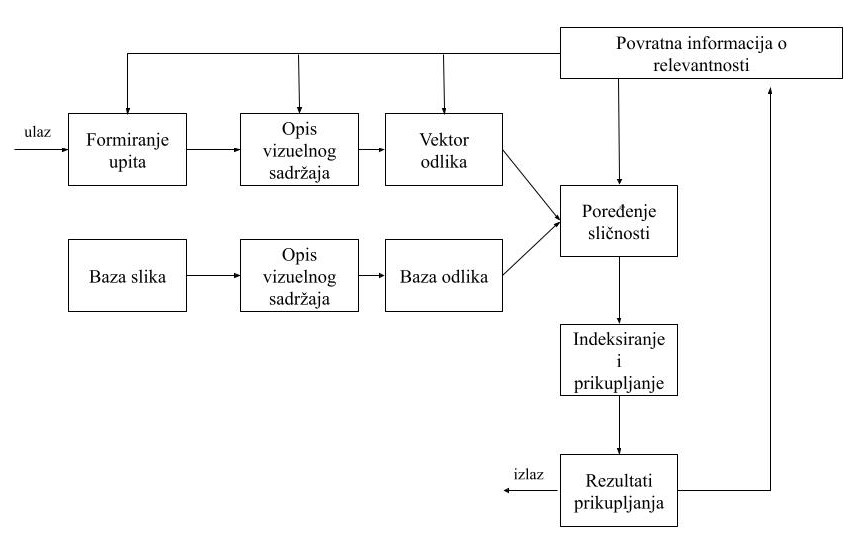
\includegraphics[width=10cm]{SZPSP.jpg}
    \caption \protect{Shematski prikaz sistema za pretragu slika po sadržaju \footnotemark[1].}
    \label{szpsp}
\end{figure}
\footnotetext[1]{Shema je preuzeta iz \cite{long2003fundamentals}.} 

Sadržaj slike može biti vizuelni i semantički. Vizuelni sadržaj može biti opšti ili vezan za određeni domen.
Opšti vizuelni sadržaj(odlike niskog nivoa) obuhvata boju, teksturu itd., dok sadržaj vezan za domen (npr. ljudsko lice) zavisi od primene i zahteva poznavanje domena.
Semantički sadržaj se dobija iz tekstualnih anotacija ili kompleksnih procedura zaključivanja na osnovu vizuelnog sadržaja \cite{long2003fundamentals}.

\section{Odlike niskog nivoa}
Izdvajanje odlika niskog nivoa pretstavlja osnovu PSPS sistema. Izdvajanje se moze izvršiti sa cele slike ili sa nekog regiona slike. Predstavljanje slika na nivou regiona je sličnije ljudskom sistemu za opažanje i samim tim više PSPS sitema koristi taj pristup. Da bi se izvršila pretraga slika zasnovanim na regionima (PSZR), prvi korak je segmentacija slike a potom se izdvajaju odlike niskog nivoa kao što su boja, tekstura, oblik ili prostorne odlike.

\subsection{Segmentacija slike}
Za segmentaciju slika postoji više algoritama, svaki ima svoje prednosti i mane. Neki od njih su:
\begin{enumerate}
\item JSEG segmentacija: sastoji iz 2 koraka - klasifikacija boja na slici i zamena piksela slike sa određeno klasom boje. Ovaj algoritam je dobar za izvlačenje sličnih tekstura i boja sa slike.
\item KMCC segmentacija - bazirano na algoritmu za klasterovanje k-sredina. Ovaj algoritam je bolji ukoliko imamo objekte na slici koji nisu homogeni a želimo da pripadaju istom regionu.
\end{enumerate}

\subsection{Odlike boja}
Boja je jedna od najčešćih odlika koja se koristi za pretraživanje slika. Ona je definisana na jednom od više mogućih prostora boja. Neki od češće korišćenih prostora boja su RGB, LAB, LUV, HSV, YCrCb i HMMD. Neke odlike boja koje se koriste u PSZR su matrica kovarijanse boja, histogram boje, momenti boje, prosečna boja i dominantna boja. Odabir odlike boje uveliko zavisi od rezultata segmentacije. Na primer ukoliko segmentacijom dobijemo nehomogene regione, proseča boja nam neće puno pomoći u ovom slučaju.

\subsection{Odlike teksture}
Tekstura nam daje bitne informacije za klasifikovanje slika. Neke češće koršćene odlika u PSPS sistemima su: spektralne odlike dobijene korišćenjen Gaborovim filtriranjem, statističke odlike kojima pripadaju 6 Tamurinih odlika i globalne odlike koje je predložio Liu et al?.

\subsection{Odlike oblika}
Oblik nije toliko korišćen u PSZR sistemima kao boja i tekstura, obično je koristan u nekik domensko specifičnim slikama kao što su objekti koje je napravio čovek. Neke osnovne odlike su odnos visine i širine, zaobljenost, Furijeovi deskriptori i uzastopna granica.

\subsection{Prostorne odlike}
Prostorne odlike su korisne u klasifikaciji regiona. Na primer more i nebo imaju sličnu boju i teksturu, ali prostorno nebo se obično nalazi na vrhu slike dok je more obično na dnu slike. Lokacija se obično jednostavno definiše kao gore ili dole. Postoje i relativni prostorni odnosi kao što su levo/desno i iznad/ispod koji se definišu za neka dva objekta.

\subsection{Mere sličnosti}
U PSZR sistemi sličnost se meri na dva nivoa. Prvi je nivo regiona koji meri sličnost 2 regiona na osnovu njihovih odlika niskog nivoa. Drugi je nivo slike koji meri sličnost 2 slike sa različitim brojem regiona. Većina istraživača koriste rastojanje Minkovskog. Ako su dva regiona predstavljena sa dva \textit{p} dimenziona vektora \textit{$(x_{1},x_{2},...,x_{p}), (y_{1},y_{2},...,y_{p})$}, redom. Onda se rastojanje Minkovskog definiše kao
$$ d(X,Y) = (\sum_{i=1}^{p} {|x_{i}-y_{i}|}^{r})^{1/r} $$
U slučaju da je $r=2$ dobijamo Euklidsko rastojanje, a ako je $r=1$ dobijamo Menhetn rastojanje.

\section{Interakcija korsnika}
U PSPS sistemima, interakcija sa korisnicima je od krucijalnog značaja, jer fleksibilnost formulacije i modifikacije upita se može postići uključivanjem korisnika u proces prikupljanja. Korisnički interfejs u ovim sistemima se najčešće sastoji od formulacije upit i prezentacije rezultat.

\subsection{Formiranje upita}
Specifikacija tipa slika koje korisnik želi da prikupi iz baze se može vršiti na više načina. Najčešće korišćeni upiti su:

\begin{enumerate}
\item \textit{Pretraživanje po kategorijama (category browsing)} - koristi se za pretraživanje baze podataka na osnovu kategorija slike. Za ovu svrhu se vrši klasifikacija slika u bazi u različite kategorije na osnovu njihovih semantičkih odlika ili na osnovu vizuelnog sadržaja.

\item \textit{Pretraživanje na osnovu koncepta (query by concept)} - koristi se za prikupljanje slika na osnovu konceptualnog opisa povezanog sa svakom slikom u bazi podataka.  
\item \textit{Pretraživanje na osnovu skice (query by sketch)} - omogućava korisniku da nacrta skicu slike koristeći alat za grafički prikaz koji ne mora biti u okviru sistema za prikupljanje.  
\item \textit{Pretraživanje na osnovu primera (query by example)} - omogućava korisniku da formuliše uput na osnovu primera slike. Sistem prevodi primer slike u unutrašnju reprezentaciju odlika. Zatim se pretražuju slike u bazi sa sličnim odlikama.

Takođe u nekim sistemima postoji mogućnost pretraživanja uz pomoć grupe slika. Sistem tada pronalazi slike koje najviše odgovaraju odlikama zadate grupe.
Mnogi sistemi omogućavaju upite sa pozitivnim i negativnim primerima \cite{long2003fundamentals}.
\end{enumerate}


\subsection{Korisnička povratna informacija}
Ljudska percepcija sličnosti između slika je subjektivna i zavisi od semantike. Iako PSPS metode daju obećavajuče rezultate za prikupljenje slika, rezultati zasnovani na sličnostima vizuelnih odlika nisu uvek percepciono i semantički značajni. Dodatno, svaki tip vizualne odlike obuhvata samo jedan aspekt svojstva slike, i korisnik često ima poteškoće da specifikuje kako se različiti aspekti kombinuju. U cilju rešavanja ovog problema, uvedena je interaktivna povratna informacija relevantnosti - tehnika iz tradicionalnih sistema za prikupljanje tekstualnih informacija. 
Primena povratne informacije omogućava uspostavljanje veze između koncepata visokog nivoa i odlika niskog nivoa.

Povratna informacija je nadgledana tehnika učenja koja se koristi za poboljšanje efikasnosti informacionih sistema. Glavna ideja je da se za unapređenje sistema koriste pozitivni i negativni primeri korisnika. Za dati upit, sistem prvobitno prikuplja listu slika na osnovu predefinisanih mera sličnosti. Zatim, korisnik označava prikupljene slike kao relevantne upitu (pozitivni primeri) ili nerelevantne (negativni primeri). Sistem će zatim uzeti u obzir i korisničke povratne informacije. Glavni problem je kako inkorporirati pozitivne i negativne primere u prečišćavanje upita i/ili njihovo uključivanje u mere sličnosti.

\section{Evaluacija performansi}
Za evaluaciju perforamsi sistema za prikupljenje koriste se dve mere
- odziv i preciznost \cite{smeulders2000content}. Skup slika iz baze koji su relevantni za dati upit q, označavamo sa $R(q)$, a prikupljene rezultate upita q sa $Q(q)$.

Preciznost prikupljenih rezultata definišemo kao razlomak prikupljenih slika koje su zaista relevantne za upit.

$$precision = \frac{ |Q(q) \cap R(q)|}{|Q(q)|}$$ \\

Odziv prikupljenih rezultata definišemo kao razlomak relevantnih slika koje je sistem prikupio na osnovu upita q.

$$recall = \frac{ |Q(q) \cap R(q)|}{|R(q)|}$$ \\

Potrebno je napraviti balans između ove dve mere, jer poboljšanjem jedne žrtvujemo drugu. U klasičnim sistemima, odziv se povećava sa povećanjem brojem prikupljenih slika, dok se preciznost u tom slučaju smanjuje. Dodatno, određivanje relevantnog skupa slika $R(q)$ je manje stabilno, zbog različitih interpretacija slika. Takođe, ukoliko je broj relevantnih slika veći nego broj prikupljenih slika, odziv je beznačajan. Dakle, preciznost i odziv predstavljaju grub opis performansi.

Iz tog razloga je predložena nova mera performansi - average normalized modified retrieval rank (ANMRR), koja kombinuje preciznost i odziv. 

Obeležimo ukupan broj slika relevantnih za upit q sa $N(q)$, a maksimalan broj relevantnih slika za svih Q upita  $ max(N(q1), N(q2), ..., N(Q)) $ sa $M$.
Onda za svaki dati uput q, svakoj relevantnoj slici $k$ se dodeljuje rang vrednosti $rank(k)$ koja je jednaka rangu $K$ ukoliko se nalazi u prvih K (gde je $K + min[4N(q), 2M])$ rezultata upita $q$. Inače joj se dodeljuje rang $K+1$.

Srednja vrednost ranga ($average rank - AVR$) za upit $q$ se računa: 

$$ AVR(q) = \sum_{k=1}^{N(q)} {\frac{rank(k)}{N(q)}}$$

Modifikovani rang ($The modified retrieval rank - MRR$) za upit q:

$$ MRR(q) = AVR(q) - 0.5 - 0.5*N(q)$$
Vrednost MMR(q) ima vrednost 0 kada se sve relevantni slike nalaze u prvih $K$ prikupljenih rezultata.

Dalje normalizujemo MMR, i dobijamo vrednosti izmđu 0 i 1:

$$ NMRR(q) = \frac{MMR(q)}{K + 0.5 + 0.5*N(q)}$$

I na kraju izvršimo usrednjavanje po svim upitima q:

$$ ANMRR = \frac{1}{Q} \sum_{q=1}^{Q} {NMRR(q)}$$

Detaljnije o ovoj meri evaluacije se može naći u \cite{long2003fundamentals}.

\section{Zaključak}



\newpage
\bibliographystyle{plain}
\bibliography{literatura.bib}

\end{document}
